\capitulo{4}{Técnicas y herramientas}

%Esta parte de la memoria tiene como objetivo presentar las técnicas metodológicas y las herramientas de desarrollo que se han utilizado para llevar a cabo el proyecto. Si se han estudiado diferentes alternativas de metodologías, herramientas, bibliotecas se puede hacer un resumen de los aspectos más destacados de cada alternativa, incluyendo comparativas entre las distintas opciones y una justificación de las elecciones realizadas. 
%No se pretende que este apartado se convierta en un capítulo de un libro dedicado a cada una de las alternativas, sino comentar los aspectos más destacados de cada opción, con un repaso somero a los fundamentos esenciales y referencias bibliográficas para que el lector pueda ampliar su conocimiento sobre el tema.
A continuación se muestran las diferentes técnicas y herramientas empleadas en el proyecto.

\section{Herramientas utilizadas}

En esta sección se describen brevemente las herramientas utilizadas en el desarrollo del proyecto. La elección de las herramientas condicionada por el desarrollo previo, ha sido actualizada con versiones más recientes. En esta sección también se describen las notas de las acciones llevadas a cabo en durante el proceso de actualización. 
Se podrá encontrar más información acerca del código y las herramientas utilizadas en el 
`Apéndice D - Documentación técnica de programación'.


\subsection{Entorno de desarrollo}\label{sect:4_1_1_HerramientasDesarrollo}
El entorno de desarrollo lo componen las diferentes herramientas que se utilizan para realizar y facilitar el desarrollo del software,

\begin{description}
	\item[\textit{Eclipse IDE for Java EE Developers}.] Entorno de programación \textit{Java} para aplicaciones web. 
	
		Se ha utilizado la versión: 2019-03. Enlace a página de descarga:
		
		\url{https://www.eclipse.org/downloads/packages/release/2019-03}
	
		\textit{Eclipse} es uno de los \textit{IDE} (\textit{Integrated Development Environment} o entorno de desarrollo integrado por sus siglas en inglés) más empleados para el desarrollo en \textit{Java}, aunque hay otros también muy utilizados como \textit{Intellij IDEA} de \textit{JetBrains}.
		
		\textit{Eclipse IDE for Java EE Developers} es un paquete que incluye herramientas para desarrolladores de \textit{Java} que crean \textit{Java EE} y aplicaciones web, incluido un \textit{IDE} de \textit{Java}, herramientas para \textit{Java EE, JPA, JSF, Mylyn, EGit} y otros.
		
Más concretamente, el paquete incluye:
\begin{itemize}
\item \textit{Data Tools Platform}
\item \textit{Eclipse Git Team Provider}
\item \textit{Eclipse Java Development Tools}
\item \textit{Eclipse Java EE Developer Tools}
\item \textit{JavaScript Development Tools}
\item \textit{Maven Integration for Eclipse}
\item \textit{Mylyn Task List}
\item \textit{Eclipse Plug-in Development Environment}
\item \textit{Remote System Explorer}
\item \textit{Eclipse XML Editors and Tools}
\end{itemize}

Podemos obtener la versión más reciente en: \url{https://www.eclipse.org/downloads/packages/release/kepler/sr2/eclipse-ide-java-ee-developers}
		
		De forma adicional a las herramientas anteriores, es posible instalar \textbf{\textit{plugins}} para ampliar la funcionalidad. En el proyecto se han instalado los siguientes:
	\begin{itemize}
		\item \textit{YEdit} para facilitar el trabajo con ficheros con un formato especial
		\item \textit{YEdit} sirve como editor de ficheros con extensión \textit{.yml}, y ha sido utilizado para generar los archivos que se usan para configurar la integración y despliegue continuo (tanto en \textit{Gitlab} como \textit{GitHub}).
		\item \textit{Vaadin Plugin for Eclipse 4.0.2}, sirve para poder usar la herramienta \textit{Vaadin} en el entorno de Eclipse de una manera más sencilla.
	\end{itemize}
		
		Eclipse dispone de varias vistas para las diferentes tareas del proyecto, las más utilizadas han sido:
		\begin{itemize}
			\item \textbf{\textit{Java EE}}. Es la vista por defecto de este paquete de \textit{Eclipse}. Facilita el trabajo de aplicaciones web y es la vista utilizada para escribir código. Ofrece, entre otras cosas, un explorador de paquetes y vistas para trabajar con \textit{Java}.
			\item \textbf{\textit{Debug}}. La vista utilizada para depurar el programa. Sirve para ejecutar la aplicación instrucción a instrucción y detectar así un problema o \textit{bug}.
			\item \textbf{\textit{Git}}. Esta vista permite trabajar con el sistema de control de versiones \textit{Git}. Mantiene una vista con un listado de repositorios, otra que visualiza el historial de cambios de un archivo seleccionado y, la más importante, una ventana que permite visualizar los cambios realizados, indexarlos, realizar \textit{commits} y publicarlos en el repositorio remoto. Eclipse permite la integración con cualquier otra forja de repositorios como \textit{GitHub} o \textit{GitLab}.
			De forma adicional se ha trabajado con la consola de \textit{Git} para \textit{Windows} \textit{GitBash}.
		\end{itemize}
		
	\item[\textit{Java SE 11 (JDK)}.] \textit{Java Development Kit}. Conjunto de herramientas software útiles para el desarrollo de aplicaciones en \textit{Java} entre las que se incluyen \textit{javac.exe}, el compilador de \textit{Java}; \textit{javadoc.exe}, el generador de documentación; y \textit{java.exe}, el intérprete de \textit{Java}.
	
		Se ha utilizado la versión  v11.0.1. Enlace a página de descarga:
		
		\url{https://www.oracle.com/java/technologies/downloads/}
	
		A pesar de haber utilizado la versión \textit{Java SE 11.0.2} \footnote{Actualmente ha sido lanzada la versión \textit{Java SE 17.0.2} y se esperan actualizaciones cada 6 meses.} de \textit{Java}. Sin embargo, ha sido posible compilar y ejecutar tanto las pruebas como la aplicación web con \textit{Java 8} realizando dos pequeñas modificaciones:
		\begin{itemize}
			\item De la versión 11 se ha utilizado el método \textit{isBlank()} de la clase \textit{String}. Se diferencia de \textit{isEmpty()} en que no comprueba la longitud de la cadena y devuelve \textit{true} si es 0, sino que devuelve \textit{true} si la longitud es 0 o si no es 0 pero todos los caracteres de la cadena son espacios en blanco.
			\item De la clase \textit{java.util.Optional} \footnote{\url{https://docs.oracle.com/en/java/javase/11/docs/api/java.base/java/util/Optional.html}}, soportada desde la versión 1.8, se utiliza la función \textit{orElseThrow()}, que se soporta desde la versión 10, por tanto habría que buscar una alternativa para pasar a la versión 1.8. La versión 11 trae a esta clase la función \textit{isEmpty()}.
		\end{itemize}
	\item[\textit{Apache Maven}.] Gestor de proyectos software que ayuda en la construcción del proyecto, la generación de documentación, generación de informes, gestión de dependencias, integración continua dentro de forjas de repositorios como \textit{GitHub} y \textit{GitLab}, etc. 
	
		Se ha actualizado a la versión v3.8.0 desde la versión  v3.8.4 que utilizaba el proyecto original \cite{TFGPrevio}. Enlace a página de descarga:
		
		\url{https://maven.apache.org/download.cgi}
		
		Se han automatizado en este proyecto utilizando \textit{Maven} y la integración continua de \textit{GitHub} (\textit{Github Actions}) los siguientes procesos:
		\begin{itemize}
			\item Compilación. Es un proceso de generación de binarios a partir del código fuente escrito en Java.
			\item Pruebas unitarias y de integración automáticas con \textit{JUnit}.
			\item Generación de informes de pruebas, cobertura con ayuda de \textit{Jacoco} y \textit{JUnit}.
			\item Despliegue en servidor de \textit{Heroku}.
		\end{itemize}
	
	\item[\textit{Maven Jetty Plugin}.] Contenedor de aplicaciones Web integrado con \textit{Maven} en forma de \textit{plugin}.
	
		Se ha utilizado la versión  v9.4.36 y se ha incluido en el proyecto en el \textit{pom.xml}:
	
\begin{verbatim}
...
<plugin>
	<groupId>org.eclipse.jetty</groupId>
	<artifactId>jetty-maven-plugin</artifactId>
	<version>9.4.36.v20210114</version>
	<configuration>
		<scanIntervalSeconds>2</scanIntervalSeconds>
	</configuration>
</plugin>
...
\end{verbatim}
		
Enlace a página de descarga:
		
		\url{https://mvnrepository.com/artifact/org.eclipse.jetty/jetty-maven-plugin/9.4.36.v20210114}
		
Se ha utilizado para desplegar en el equipo local de desarrollo y realizar pruebas durante el desarrollo en local. Para correr la aplicación en el entorno local basta con ejecutar: 
		
\begin{verbatim}
mvn jetty:run
\end{verbatim}

y gracias a la capacidad que tiene el \textit{plugin} de captar los cambios (cada dos segundos según podemos ver en la configuración previa) facilita mucho el desarrollo al recompilar automáticamente el proyecto.
		
\end{description}
\subsection{\textit{Logging}}
El \textit{logging} es el proceso que permite ver lo que ocurre durante la ejecución de la aplicación para poder depurar errores y analizar comportamientos para solucionar diferentes problemas. Este proceso es útil tanto en la fase de desarrollo del proyecto como en la de producción una vez la aplicación está desplegada y en uso por usuarios finales.

\begin{description}
	\item[\textit{SLF4J}.] Visualización del \textit{logging}.
	Sirve como una simple fachada o abstracción para varios marcos de registro (por ejemplo, \textit{java.util.logging, logback, log4j}) que permite al usuario final conectar el marco de registro deseado en el momento de la implementación.
	
		Enlace a página de descarga:
	
		\url{https://www.slf4j.org/download.html}
	
	\item[\textit{Log4j 2}.] \textit{Logger}. Se ha utilizado actualizado la versión a la 2.17.2 desde v2.11.2 utilizada por el proyecto previo \cite{TFGPrevio} para evitar diferentes vulnerabilidades.

	 	Enlace a página de descarga:
	
	 	\url{https://mvnrepository.com/artifact/org.apache.logging.log4j/log4j-core/2.17.2}\\
		
		Esta herramienta permite configurar este proceso por medio de un fichero \textit{log4j2} con extensión \textit{XML}, \textit{JSON}, \textit{YAML} o \textit{Properties}\footnote{Manual de configuración de \textit{Log4j 2}: \url{https://logging.apache.org/log4j/2.x/manual/configuration.html}} \cite{apache_apache_nodate}. En este proyecto se configuró mediante un fichero con extensión \textit{.properties}. 
		
		Ambas herramientas están integradas con \textit{Maven}, y sólo es necesario añadir en el fichero \ruta{pom.xml} las dependencias correspondientes.
	
\end{description}
\subsection{Pruebas}
La fase de pruebas permite comprobar que la implementación realizada funciona correctamente y no contiene errores. Se han implementado dos tipos de pruebas: unitarias y de integración. Las unitarias prueban los diferentes módulos y las de integración prueban la relación que tienen los diferentes módulos entre sí.
\begin{description}
	\item[JUnit5]. Conjunto de bibliotecas para el desarrollo de pruebas unitarias. 
	
		Se ha utilizado la versión  v5.3.1. Enlace a página de descarga:
		
		\url{https://junit.org/junit5/}
		
		\textit{JUnit} permite realizar pruebas unitarias de forma automática o semiautomática de aplicaciones \textit{Java}. Se han ejecutado de ambas formas en el proyecto. La automatización completa ha sido posible gracias a las herramientas de \textit{CI} (\textit{Continuous Integration}) de \textit{Github} \textit{GitHub Actions}: 
		\url{https://docs.github.com/es/actions}
		
		Esta versión de \textit{JUnit 5}, sobre la anterior \textit{JUnit 4}, ha influido en este proyecto de la siguiente manera:
		\begin{itemize}
			\item \textit{JUnit 5} soporta \textbf{Java 11}.
			
			\item Permite realizar asertos (\textit{asserts}) de tipo \textit{\textbf{assertAll()}} \footnote{\url{https://junit.org/junit5/docs/current/api/org/junit/jupiter/api/Assertions.html}}. Este tipo de asertos permite tratar varios asertos como una unidad. Se utilizaron en versiones anteriores de la aplicación, pero realmente no eran necesarios y se optó por quitarlos.
			
			\item Permite realizar \textbf{comprobaciones de lanzamiento de excepciones} en asertos del tipo \textit{assertThrows()}.
			
			\item Permite realizar suposiciones (\textit{\textbf{assumptions}}) que permiten realizar una comprobación que pasará por alto un test (lo marca como \textit{skipped}) si la comprobación falla. Es decir, que no lo marcará como error, simplemente no realizará el test. 
			\\Esto ha sido útil de cara a probar funciones que realizan conexiones a \textit{GitLab} o \textit{GitHub} que requieren credenciales de acceso que no se pueden publicar en los test ya que quedarían publicadas. Por tanto estos test tienen presunciones que comprueban que se tiene las credenciales de acceso y no se realizan los test si no se dispone de estas credenciales, en lugar de lanzar un error por no poder realizar la conexión.
			\\Estos test se ejecutan manualmente por el programador en su equipo local y no se ejecutan automáticamente en el proceso de integración continua.
			
			\item Permite crear \textbf{tests parametrizados}. Estos son test que prueban funciones que requieren argumentos. Cada combinación de argumentos es un caso de prueba, y crear un test para cada combinación es un caso claro del defecto de código: `código duplicado'. Por ello estos argumentos se pueden generar mediante funciones, enumeraciones, proveedores de argumentos o recolectar desde un \textit{CSV} y solo ser necesario un test para todas las combinaciones de argumentos posibles.
		\end{itemize}
\end{description}
\subsection{Frameworks y librerías específicas para el proyecto}
\begin{description}
	\item[\textit{github-api.kohsuke}]. Librería de conexión a \textit{GitHub API}. 
	
		Se ha utilizado esta librería para realizar la conexión con la \textit{API} de \textit{GitHub} en su última versión disponible, la 1.306:
		
		\url{https://github-api.kohsuke.org/}
		
		
	\item[\textit{gitlab4j-api}]. \textit{Framework} de conexión a \textit{GitLab API}. 
	
		Se ha actualizado a última versión disponible, la versión  v4.19.0. Enlace:
		
	\url{https://javadoc.io/doc/org.gitlab4j/gitlab4j-api/4.19.0/index.html}
		
		
			
	\item[\textit{Apache Commons Math}]. Librería que se utiliza para matemáticas descriptivas y que ha servido para el cálculo de cuartiles, necesarios para obtener los valores umbrales de las métricas según las estadísticas. 
	
		Se ha utilizado la versión  v3.6.1. Enlace a página de descarga:
	
		\url{https://commons.apache.org/proper/commons-math/download_math.cgi}
		
		Ejemplo de uso de la clase \textit{DescriptiveStatistics} de la librería:
		
\begin{minipage}{\linewidth}
{\tiny 
\begin{verbatim}[breaklines]
...
ArrayList<Double> datasetForMetric;
Double q1ForMetric, q3ForMetric;
DescriptiveStatistics descriptiveStatisticsForMetric;

descriptiveStatisticsForMetric = new DescriptiveStatistics(datasetForMetric
	  .stream()
	  .mapToDouble(x -> x)
	  .toArray());
q1ForMetric = descriptiveStatisticsForMetric.getPercentile(25);
q3ForMetric = descriptiveStatisticsForMetric.getPercentile(75);
...
\end{verbatim}
}
\end{minipage}		

\end{description}
\subsection{Interfaz gráfica}
\begin{description}
	\item[\textit{Vaadin}]. \textit{Framework} para desarrollo de interfaces web con \textit{Java}.
		Se ha utilizado la versión  v13.0.0 Enlace:
		
		\url{https://vaadin.com/}
		
		Con este framework no ha sido necesario escribir \textit{HTML}, solo \textit{Java} y \textit{CSS} para los estilos. 
		\\Como ejemplo de esto, para implementar un \textit{input} se utilizaría el siguiente código:
		
\begin{minipage}{\linewidth}
\tiny \begin{verbatim}
...
EmailField emailField = new EmailField();
emailField.setLabel("Email address");
add(emailField);
...
\end{verbatim}
\end{minipage}	

		y el resultado sería el de las siguientes figuras Fig. \ref{fig:M4_Vaadin_Input_1} y Fig. \ref{fig:M4_Vaadin_Input_2}
\begin{figure}[!h]
	\centering
	
\includegraphics[scale=0.5]{M4_Vaadin_Input_1}
	\caption{\textit{Input} generado por \textit{Vaadin} vacío}\label{fig:M4_Vaadin_Input_1}
	
	
	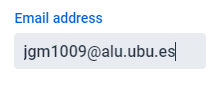
\includegraphics[scale=0.5]{M4_Vaadin_Input_2}
	\caption{\textit{Input} generado por \textit{Vaadin} con texto}\label{fig:M4_Vaadin_Input_2}
\end{figure}
\FloatBarrier

\end{description}
\subsection{Desarrollo y despliegue continuo}
\begin{description}
	\item[\textit{GitHub}]. Forja (plataforma de desarrollo colaborativo) para alojar proyectos utilizando el sistema de control de versiones \textit{Git} en la que se ha almacenado el proyecto en un repositorio \textit{Git}.
	
		Enlace a \textit{GitHub}:
		
		\url{https://github.com/}
		
		Enlace al repositorio del proyecto:
		
		\url{https://github.com/Joaquin-GM/GII_O_MA_19.07-Comparador-de-metricas-de-evolucion-en-repositorios-Software}
		
		En este proyecto se ha optado por utilizar \textit{GitHub} frente a la primera iteración del proyecto \cite{TFGPrevio} para explorar su funcionalidad y comprobar que también es utilizable. Para más información hay una comparativa entre \textit{GitHub} y \textit{GitLab} en la sección \ref{sect:3_2_1_GitHubVSGitLab}.
		
	% \item[Codacy]. Herramienta de generación automática de informes de calidad de código.
	
	%	 Enlace a Codacy:
		 
	%	 \url{https://www.codacy.com/}
		 
	%	 Enlace a proyecto en Codacy: 
		 
		 % TODO -> cuando esté generado poner el enlace al manual del proyecto
	%	 \url{https://app.codacy.com}
	
	\item[\textit{JaCoCo}]. Librería utilizada para generar informes de cobertura del código en \textit{Java}. Estos informes se pueden mostrar en \textit{GitHub} fácilmente publicando los informes con formato \textit{HTML}. 
	%También se han enviado estos informes a Codacy para que controle la cobertura además de la calidad de código.
	
		Se ha actualizado al proyecto para usar la la versión v0.8.7. 
		
		%Enlace:
		
		%\url{https://www.eclemma.org/jacoco/}
		
		Enlace a informe de \textit{JaCoCo} en \textit{HTML} sobre la cobertura del proyecto:
		
		% TODO -> cuando esté generado el primer nuevo informe poner url
		% \url{}
	
	\item[\textit{Heroku}]. Herramienta para desplegar la aplicación (\textit{CD}).
	
		Enlace a herramienta:
		
		\url{https://id.heroku.com/login}
		
		Enlace a aplicación desplegada:
		
		\url{https://evolution-metrics-v2.herokuapp.com/}
	
\end{description}
\subsection{Documentación}
\begin{description}
	\item[\textit{LaTeX}]. Sistema de composición de textos.
		Enlace a herramienta:
		
		\url{https://www.latex-project.org/}
		
	\item[TeXMaker]. Entorno de desarrollo de documentos \textit{LaTeX}.
	
		Enlace a herramienta:
		
		\url{https://www.xm1math.net/texmaker/}
	
	\item[Zotero]. Herramienta de gestión de fuentes bibliográficas.
		
		Enlace a herramienta:
		
		\url{https://www.zotero.org/}
	
\end{description}
\section{Técnicas}
\begin{itemize}
	\item A lo largo del proyecto se han utilizado diferentes patrones de diseño \cite{gamma_patrones_2002} como \textit{Singleton, Factory Method, Wrapper, Builder, Listener}, etc.En los apéndices se puede encontrar más información al respecto.
	
	\item Para el motor de métricas se ha utilizado como base el framework propuesto en \textit{Soporte de Métricas con Independencia del Lenguaje para la Inferencia de Refactorizaciones} \cite{marticorena_sanchez_soporte_2005}. Ver Fig. \ref{fig:MCTMotorMetricas} en la sección \ref{sect:3_3_3_FrameworkMedicion}.
	
	\item El ciclo de vida del software de este proyecto se ha basado en \textit{Scrum}\cite{scrum_master_scrum_2019}, es decir, ha seguido un modelo de proceso iterativo e incremental. En el documento de anexos en su primera sección titulada Plan de proyecto se mostrarán los detalles de las iteraciones.
\end{itemize}
